\begin{appendices}

\chapter{Cut and Matching Results}
\label{App:CutAndMatchingResults}

\begin{figure}[p]
  \centering
  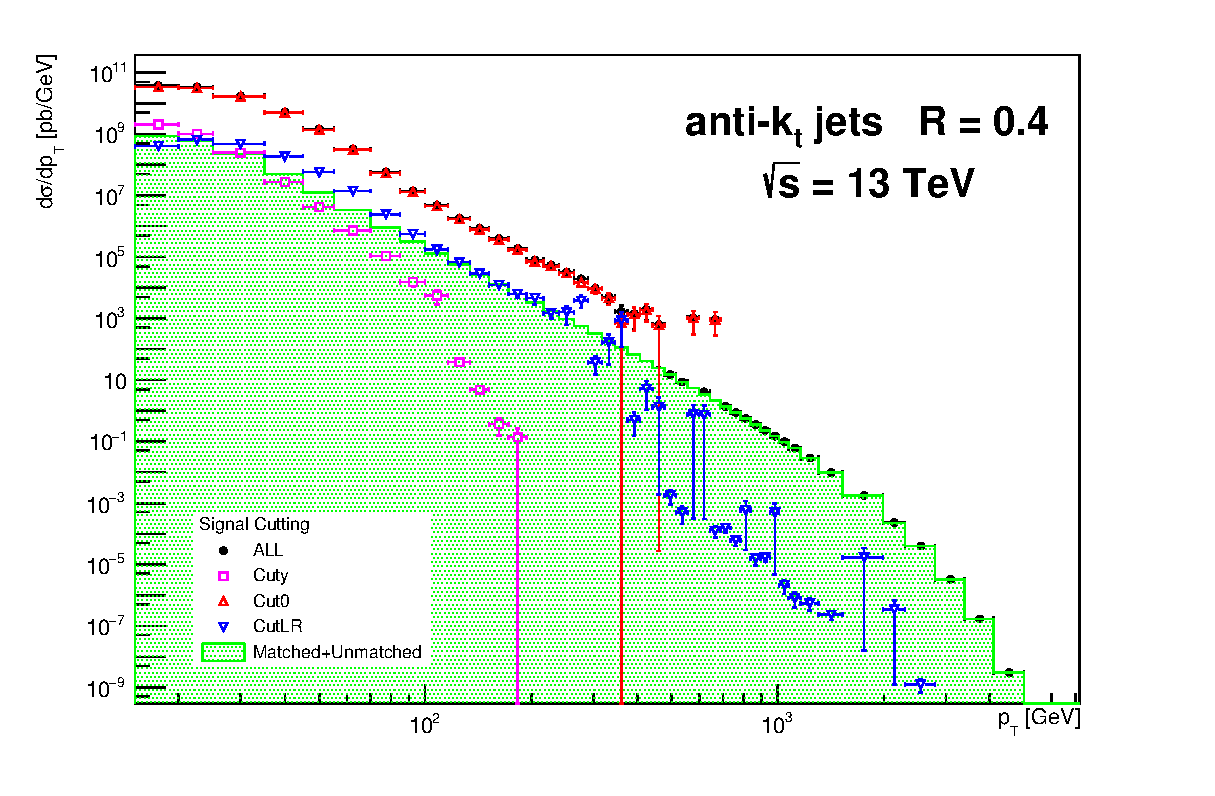
\includegraphics[width=0.9\textwidth]{Chapter3/SignalCutting.eps}
  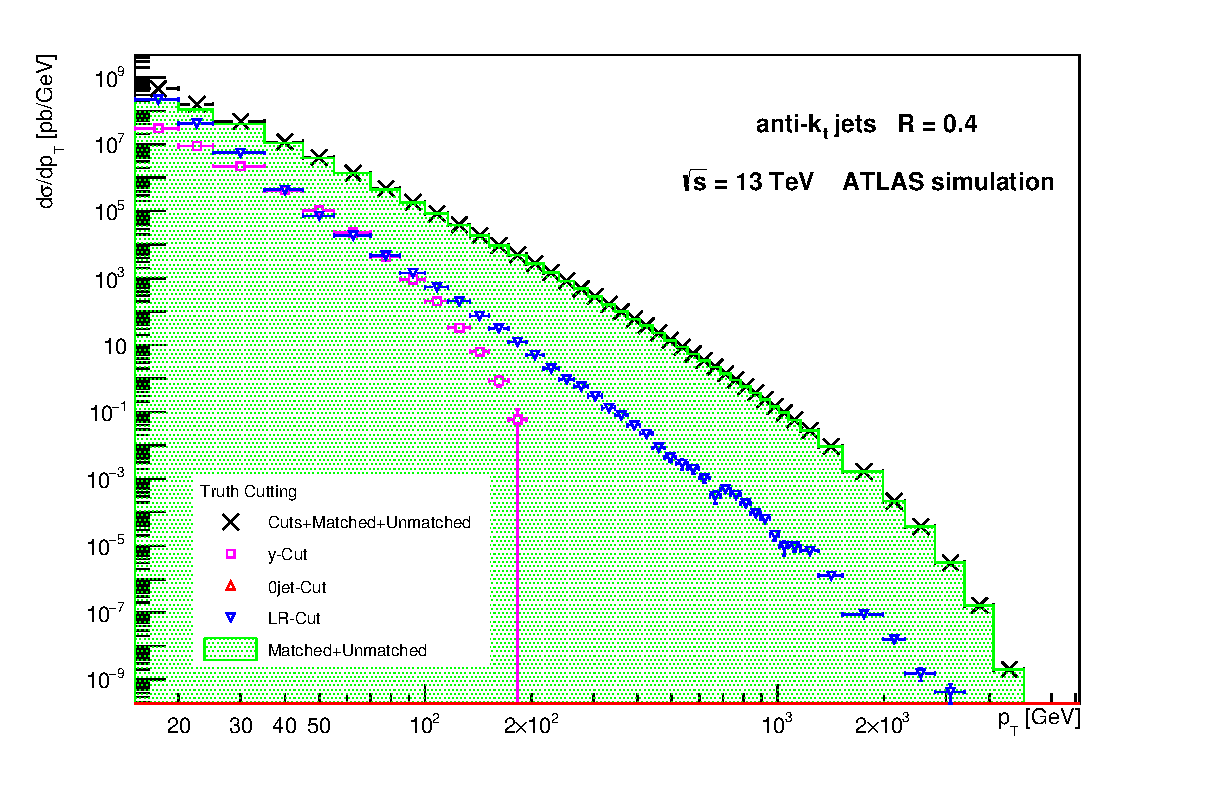
\includegraphics[width=0.9\textwidth]{Chapter3/TruthCutting.eps}
  \caption{Impact of 4 cuts defined in Section \ref{SubSec:JetCuts} on
  differential cross section in $\pt$ of signal jets (top) and truth jets
  (bottom). Black dots represent the original uncutted spectrum, green area then
  these jets, which survived all four cutoffs.}
  \label{fig:Cutting}
\end{figure}

\begin{figure}[p]
  \centering
  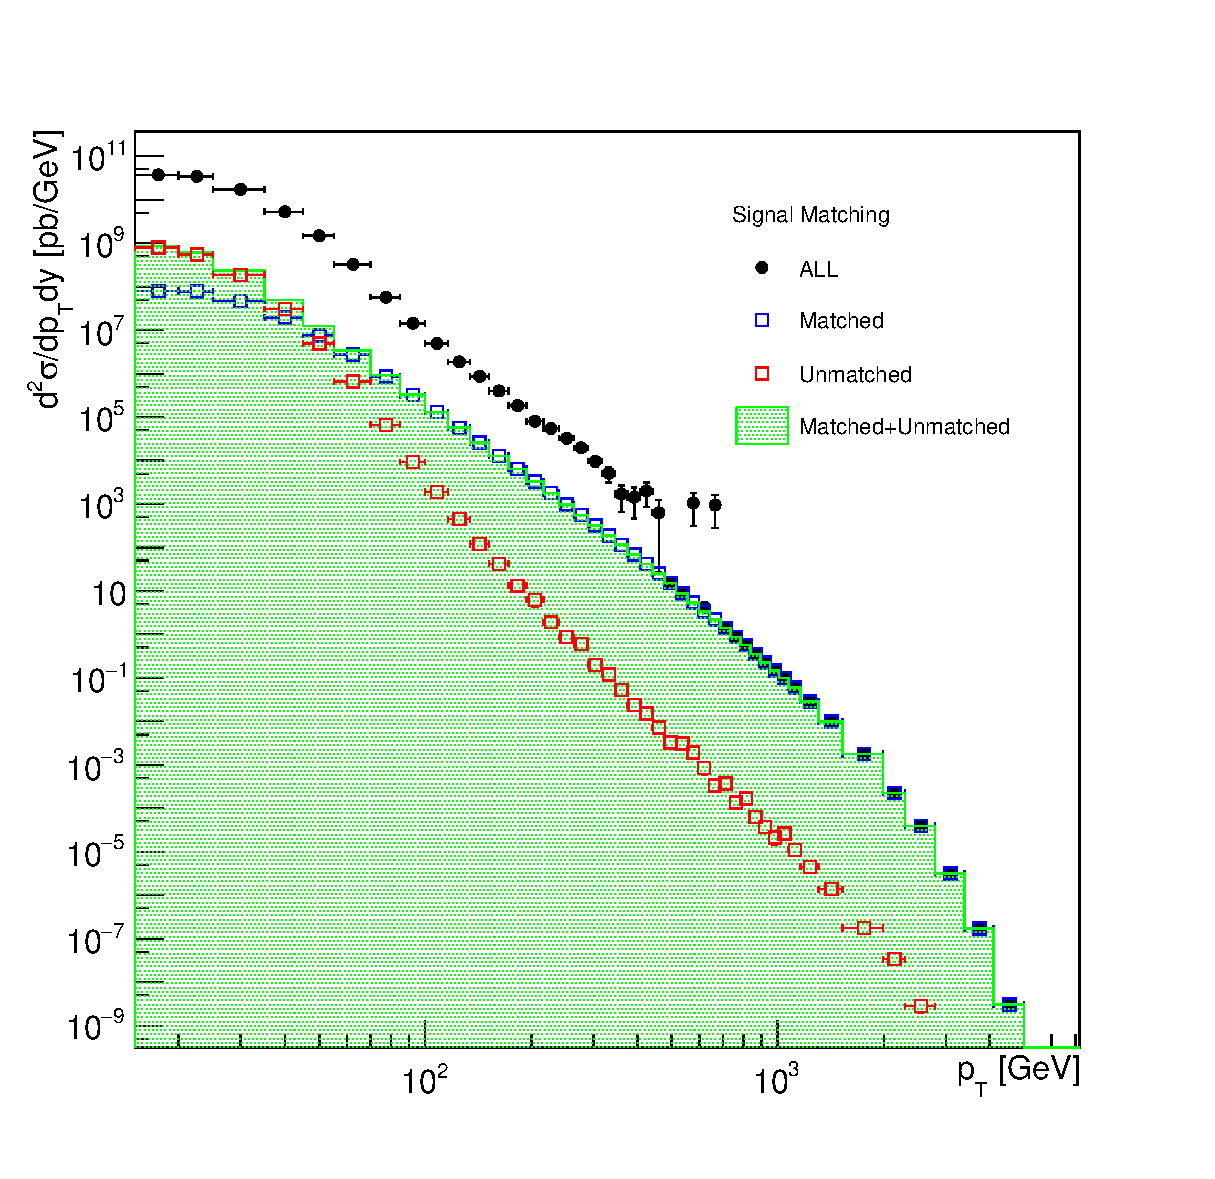
\includegraphics[width=0.9\textwidth]{Chapter3/SignalMatching.eps}
  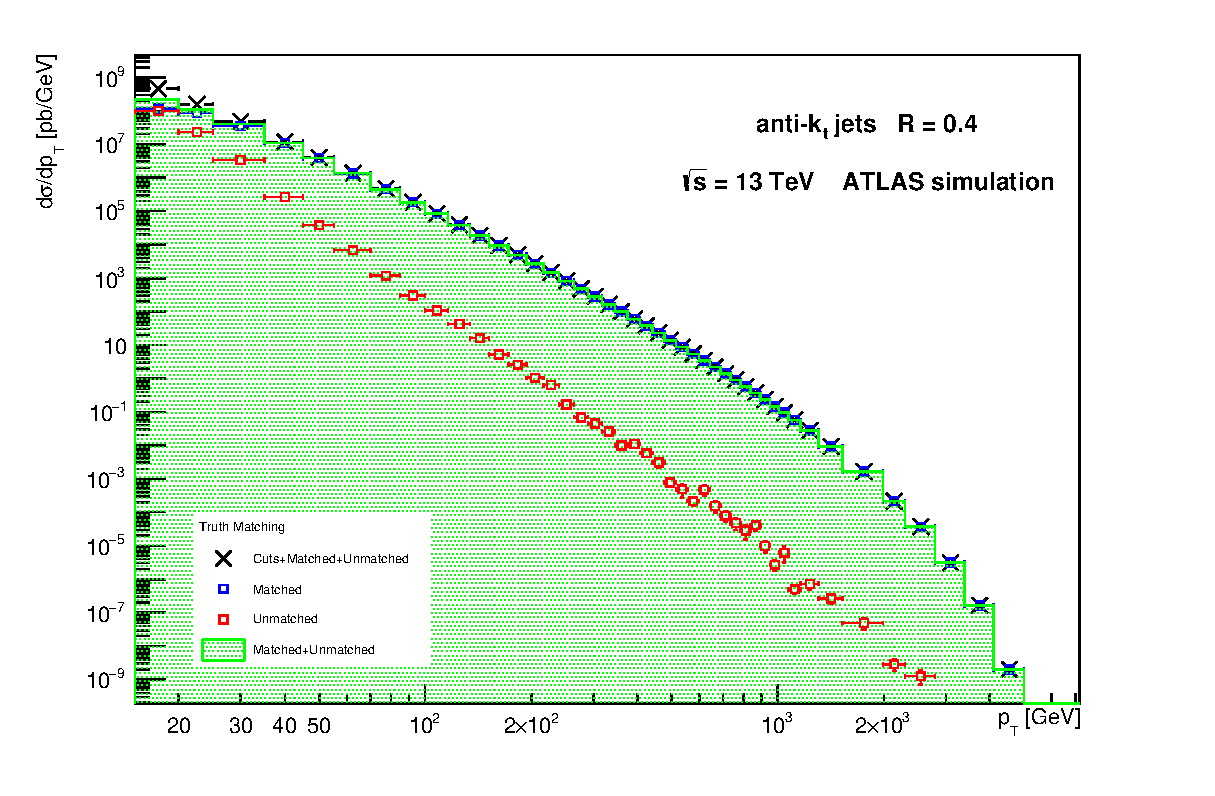
\includegraphics[width=0.9\textwidth]{Chapter3/TruthMatching.eps}
  \caption{Results of matching procedure described in Section
  \ref{SubSec:JetMatching} demonstrated on differential cross section in $\pt$ of
  signal (top) and truth (bottom) jets. Black dots represent the original
  uncutted spectrum. The contribution of matched and unmatched jets to
  green area representing all jets which survived cutoffs is shown.}
  \label{fig:Matching}
\end{figure}

\begin{figure}[p]
  \centering
  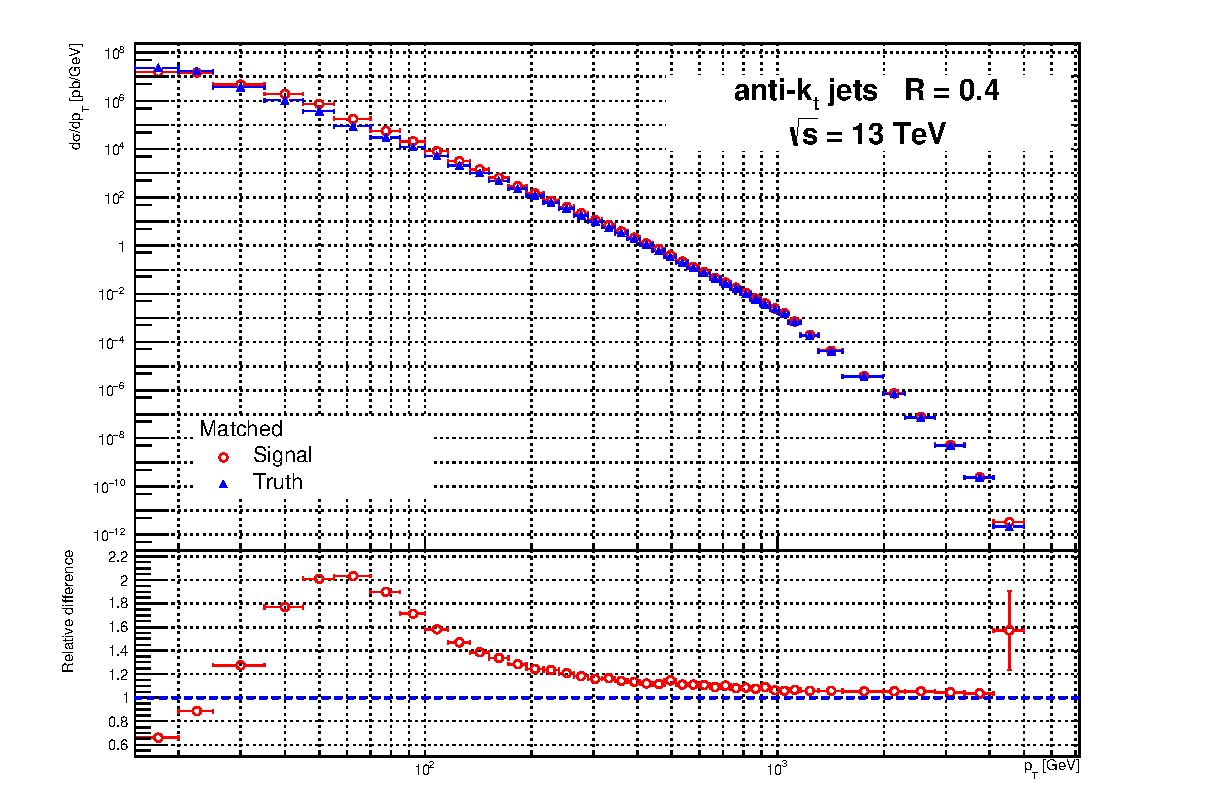
\includegraphics[width=0.9\textwidth]{Chapter3/SignalVSTruthMatched.eps}
  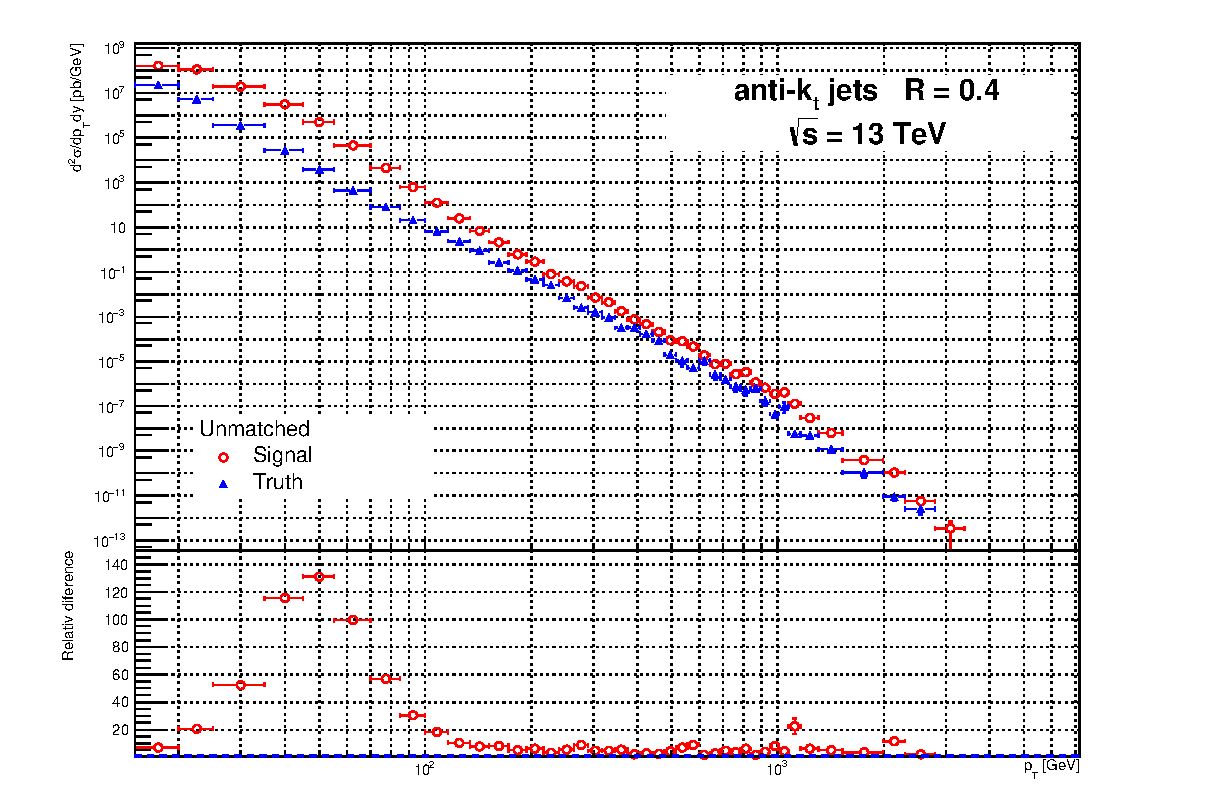
\includegraphics[width=0.9\textwidth]{Chapter3/SignalVSTruthUnmatched.eps}
  \caption{Comparison of $\pt$ spectra of matched (top) and unmatched (bottom)
  signal and truth jets. The $\pt$ spectra are the same as those at Figure
  \ref{fig:Matching}. Only difference is, that there are compared spectra of
  signal and truth jets.  The bottom part both of these graphs shows the
  relative difference between signal and truth spectrum. }
  \label{fig:MatchedUnmatched}
\end{figure}

\begin{landscape} 
\begin{table}
  \centering
  \begin{tabular}{|c|c|>{\bfseries}c|c|c|c|c|c|c|c|c|}
    \hline
     \multicolumn{2}{|c|}{\# jets}  & ALL      & JZ0W     & JZ1W     & JZ2W     & JZ3W     & JZ4W     & JZ5W     & JZ6W     & JZ7W     \\
    \hline                                                              
    \hline                                                              
     \multicolumn{2}{|c|}{Signal}   & 1.10e+08 & 3.22e+07 & 3.59e+07 & 6.67e+06 & 7.07e+06 & 6.28e+06 & 7.29e+06 & 7.13e+06 & 7.11e+06 \\
    \hline                                                              
     \multicolumn{2}{|c|}{Truth}    & 7.22e+07 & 3.15e+06 & 3.00e+07 & 6.17e+06 & 6.91e+06 & 6.20e+06 & 6.98e+06 & 6.53e+06 & 6.25e+06 \\
    \hline                                                              
    \hline                                                              
    \multirow{4}{*}{CutPt}          & \multirow{2}{*}{Signal}   & 1.32e+07 & 5.45e+06 & 4.38e+06 & 6.50e+05 & 5.87e+05 & 4.76e+05 & 5.48e+05 & 5.52e+05 & 5.63e+05 \\
                                    &                           & 12.1 \%  & 17.0 \%  & 12.2 \%  & 9.7 \%   & 8.3 \%   & 7.6 \%   & 7.5 \%   & 7.7 \%   & 7.9 \%   \\
    \cline{2-11}                                                                 
                                    & \multirow{2}{*}{Truth}    & 4.67e+07 & 3.11e+06 & 2.20e+07 & 3.86e+06 & 4.00e+06 & 3.42e+06 & 3.74e+06 & 3.43e+06 & 3.23e+06 \\
                                    &                           & 64.7 \%  & 98.7 \%  & 73.1 \%  & 62.6 \%  & 57.8 \%  & 55.1 \%  & 53.6 \%  & 52.5 \%  & 51.6 \%  \\
    \hline                                                              
    \hline                                                              
    \multirow{4}{*}{Cuty}           & \multirow{2}{*}{Signal}   & 2.46e+06 & 8.02e+05 & 9.54e+05 & 1.42e+05 & 1.28e+05 & 1.03e+05 & 1.16e+05 & 1.10e+05 & 1.08e+05 \\
                                    &                           & 2.2 \%   & 2.5 \%   & 2.7 \%   & 2.1 \%   & 1.8 \%   & 1.6 \%   & 1.6 \%   & 1.5 \%   & 1.5 \%   \\
    \cline{2-11}                                                                                    
                                    & \multirow{2}{*}{Truth}    & 5.03e+05 & 3.14e+03 & 3.19e+05 & 4.54e+04 & 3.79e+04 & 2.88e+04 & 2.78e+04 & 2.22e+04 & 1.83e+04 \\
                                    &                           & 0.7 \%   & 0.1 \%   & 1.1 \%   & 0.7 \%   & 0.5 \%   & 0.5 \%   & 0.4 \%   & 0.3 \%   & 0.3 \%   \\
    \hline                                                              
    \hline                                                              
    \multirow{4}{*}{Cut0jet}        & \multirow{2}{*}{Signal}   & 2.62e+07 & 2.56e+07 & 5.49e+05 & 0.00e+00 & 0.00e+00 & 0.00e+00 & 0.00e+00 & 0.00e+00 & 0.00e+00 \\
                                    &                           & 23.9 \%  & 79.6 \%  & 1.5 \%   & 0.0 \%   & 0.0 \%   & 0.0 \%   & 0.0 \%   & 0.0 \%   & 0.0 \%   \\
    \cline{2-11}                                                                                    
                                    & \multirow{2}{*}{Truth}    & 0.00e+00 & 0.00e+00 & 0.00e+00 & 0.00e+00 & 0.00e+00 & 0.00e+00 & 0.00e+00 & 0.00e+00 & 0.00e+00 \\
                                    &                           & 0.0 \%   & 0.0 \%   & 0.0 \%   & 0.0 \%   & 0.0 \%   & 0.0 \%   & 0.0 \%   & 0.0 \%   & 0.0 \%   \\
    \hline                                                              
    \hline                                                              
    \multirow{4}{*}{CutLR}          & \multirow{2}{*}{Signal}   & 3.64e+06 & 2.27e+05 & 3.37e+06 & 2.99e+04 & 7.07e+03 & 2.33e+03 & 1.63e+03 & 7.14e+02 & 6.31e+02 \\
                                    &                           & 3.3 \%   & 0.7 \%   & 9.4 \%   & 0.4 \%   & 0.1 \%   & 0.0 \%   & 0.0 \%   & 0.0 \%   & 0.0 \%   \\
    \cline{2-11}                                                                                    
                                    & \multirow{2}{*}{Truth}    & 5.21e+05 & 2.15e+04 & 4.74e+05 & 1.82e+04 & 4.45e+03 & 1.33e+03 & 9.03e+02 & 4.37e+02 & 2.78e+02 \\
                                    &                           & 0.7 \%   & 0.7 \%   & 1.6 \%   & 0.3 \%   & 0.1 \%   & 0.0 \%   & 0.0 \%   & 0.0 \%   & 0.0 \%   \\
    \hline                                                              
    \hline                                                              
    \multirow{4}{*}{Matched}        & \multirow{2}{*}{Signal}   & 2.13e+07 & 7.95e+03 & 5.99e+06 & 1.95e+06 & 2.54e+06 & 2.46e+06 & 2.88e+06 & 2.78e+06 & 2.72e+06 \\
                                    &                           & 19.5 \%  & 0.0 \%   & 16.7 \%  & 29.3 \%  & 36.0 \%  & 39.1 \%  & 39.5 \%  & 38.9 \%  & 38.2 \%  \\
    \cline{2-11}                                                                                    
                                    & \multirow{2}{*}{Truth}    & 2.13e+07 & 7.95e+03 & 5.99e+06 & 1.95e+06 & 2.54e+06 & 2.46e+06 & 2.88e+06 & 2.78e+06 & 2.72e+06 \\
                                    &                           & 29.5 \%  & 0.3 \%   & 19.9 \%  & 31.7 \%  & 36.8 \%  & 39.6 \%  & 41.3 \%  & 42.5 \%  & 43.5 \%  \\
    \hline                                                              
    \hline                                                              
    \multirow{4}{*}{Unmatched}      & \multirow{2}{*}{Signal}   & 4.28e+07 & 6.15e+04 & 2.06e+07 & 3.89e+06 & 3.81e+06 & 3.24e+06 & 3.75e+06 & 3.69e+06 & 3.72e+06 \\
                                    &                           & 39.0 \%  & 0.2 \%   & 57.5 \%  & 58.4 \%  & 53.8 \%  & 51.6 \%  & 51.4 \%  & 51.8 \%  & 52.3 \%  \\
    \cline{2-11}                                                                                    
                                    & \multirow{2}{*}{Truth}    & 3.14e+06 & 7.51e+03 & 1.30e+06 & 2.89e+05 & 3.29e+05 & 2.95e+05 & 3.29e+05 & 3.03e+05 & 2.88e+05 \\
                                    &                           & 4.4 \%   & 0.2 \%   & 4.3 \%   & 4.7 \%   & 4.8 \%   & 4.8 \%   & 4.7 \%   & 4.6 \%   & 4.6 \%   \\
    \hline
  \end{tabular}
  \caption{Statistics for matching and cutting procedures described in Sections
  %\ref{SubSec:JetCuts} and \ref{SubSec:JetMatching} displayed for all jets and for
  %individual JZXW samples defined in Table \ref{tab:JZXW}. At the top, there is
  %number of initial signal and truth jets respectively. For each cut, there is
  %shown the number of jets, which were killed by it, and their relative number
  %according to the original number of signal or truth jets respectively.
  %Last two lines show the statistics of matching procedure including number of
  jets which were (un)matched.}
  \label{tab:CutAndMatchingEfficiency}
\end{table} 
\end{landscape}

\chapter{Unfolding Results}
\label{App:UnfoldingResults}

\begin{figure}[h]
  \centering
  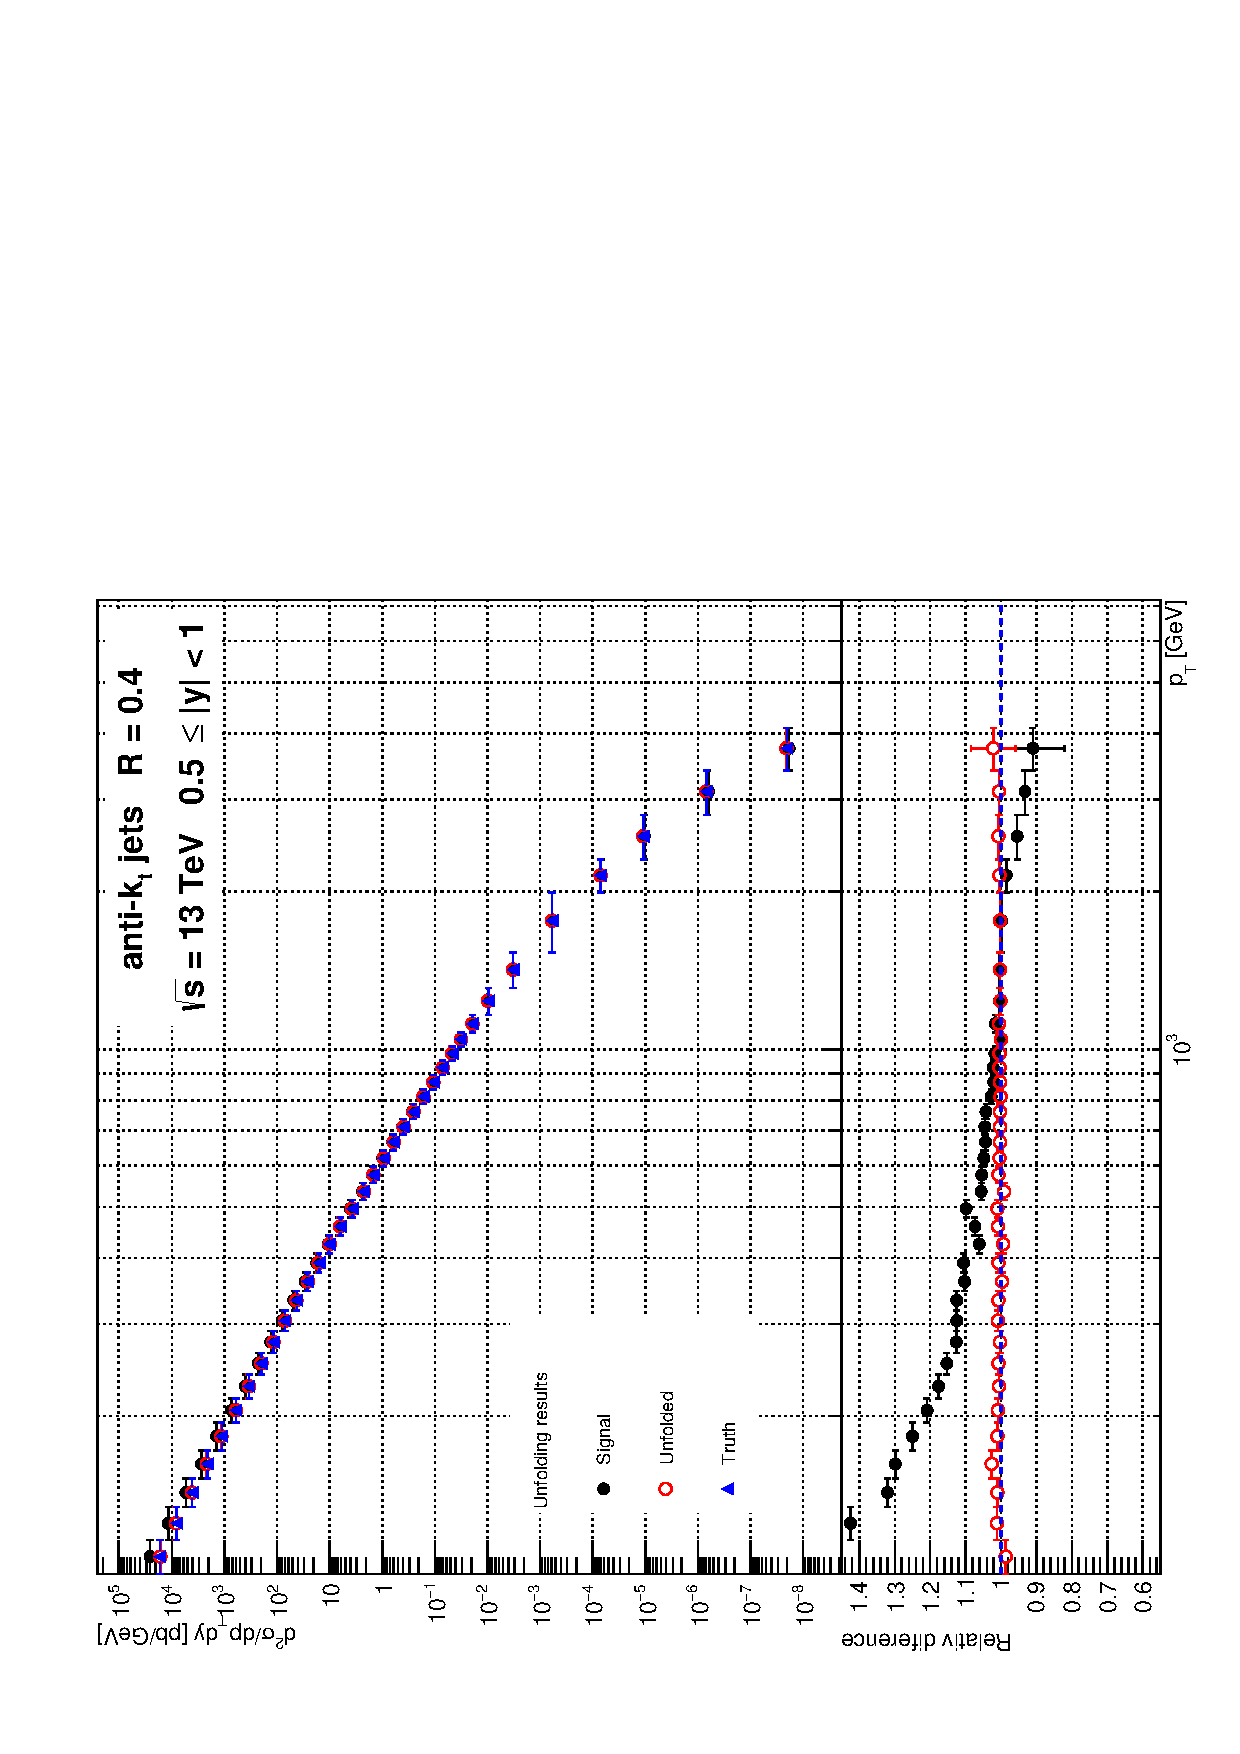
\includegraphics[width=\textwidth]{{Chapter3/Signal_VS_Unfold_VS_Truth_abs(y)0.5-1}.eps}
  \caption{Comparison of spectra of signal jets and unfolded spectra of signal
  jets with the spectrum of truth jets for $0.5 \leq |y| < 1$ rapidity bin. Each bin was
  divided by its width so the $y$-axis has meaning of double differential cross
  section in $\pt$ and $y$. The graph at bottom shows the relative difference
  between signal or unfolded spectrum and the truth spectrum.}
  \label{fig:Unfolding1}
\end{figure}

\begin{figure}[p]
  \centering
  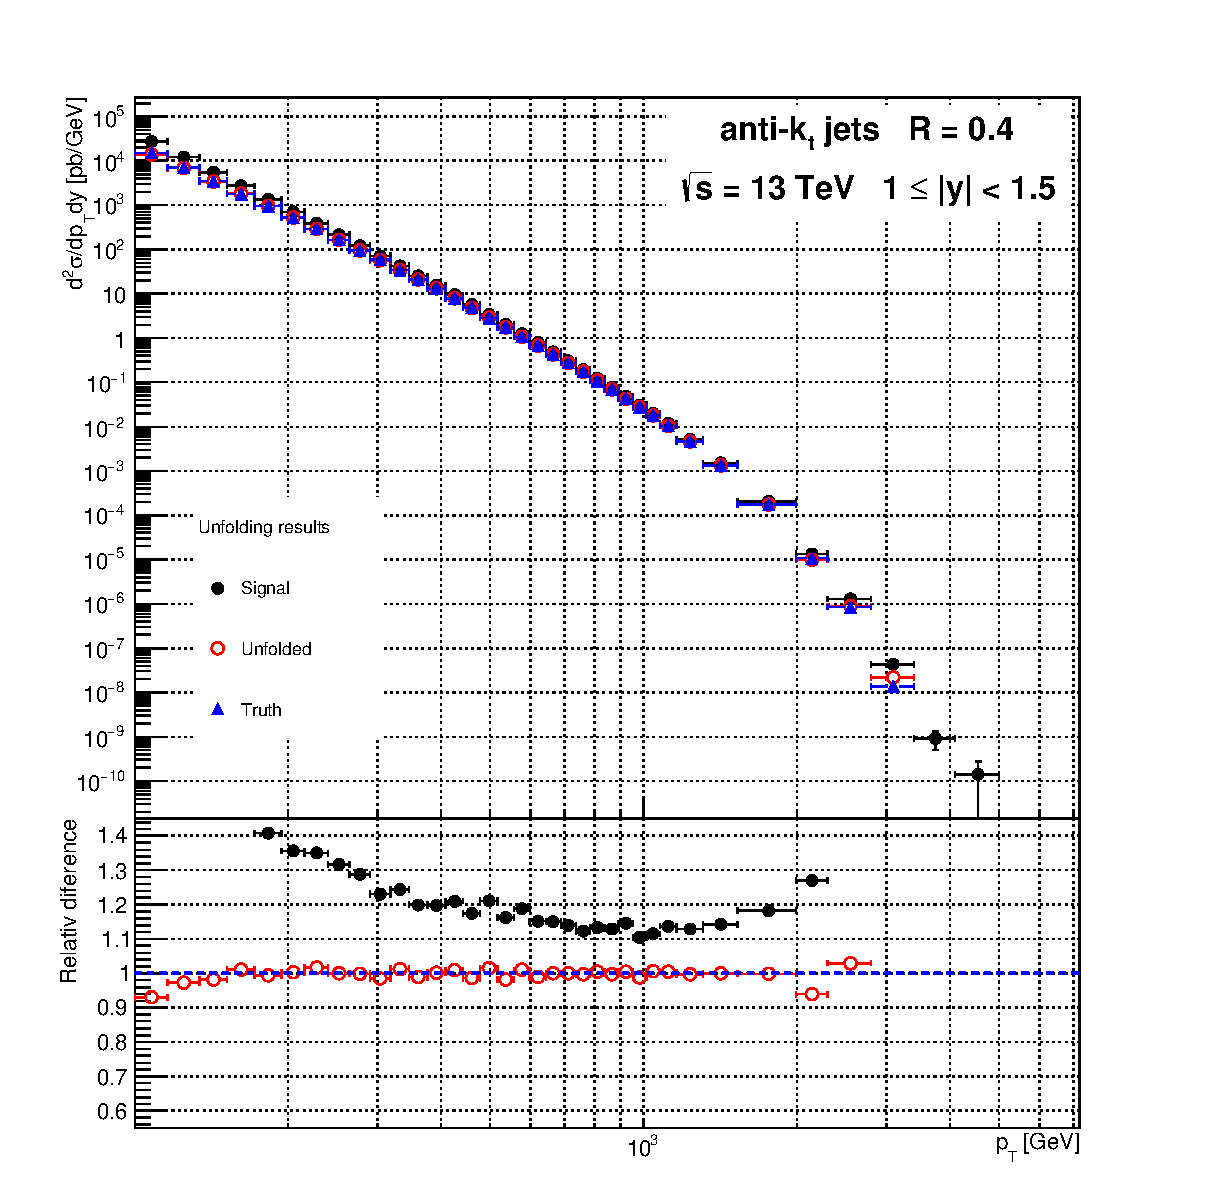
\includegraphics[width=0.9\textwidth]{{Chapter3/Signal_VS_Unfold_VS_Truth_abs(y)1-1.5}.eps}
  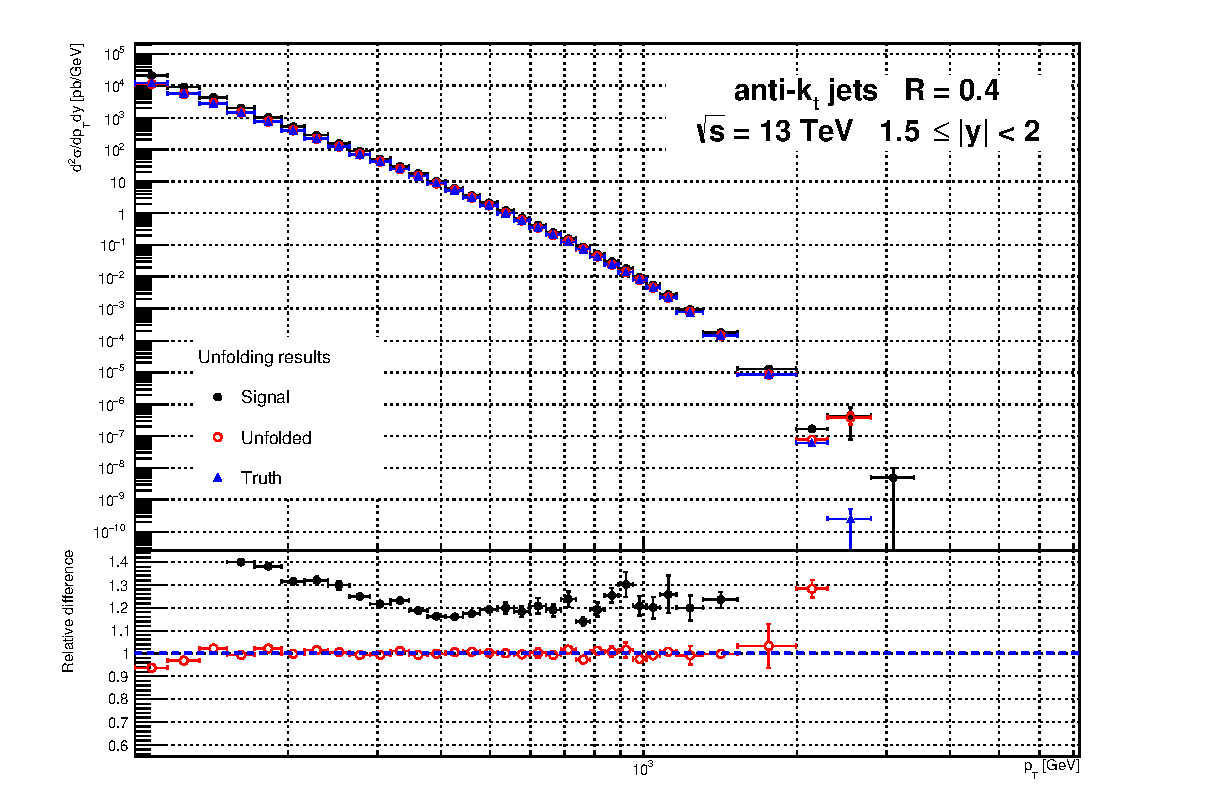
\includegraphics[width=0.9\textwidth]{{Chapter3/Signal_VS_Unfold_VS_Truth_abs(y)1.5-2}.eps}
  \caption{Comparison of spectra of signal jets and unfolded spectra of signal
  jets with the spectrum of truth jets for $1 \leq |y| < 1.5$ (top) and $1.5
  \leq |y| < 2$ (bottom) rapidity bin. Each bin was divided by its width so the
  $y$-axis has meaning of double differential cross section in $\pt$ and $y$. The
  graph at bottom shows the relative difference between signal or unfolded
  spectrum and the truth spectrum.} 
  \label{fig:Unfolding2}
\end{figure}

\begin{figure}[p]
  \centering
  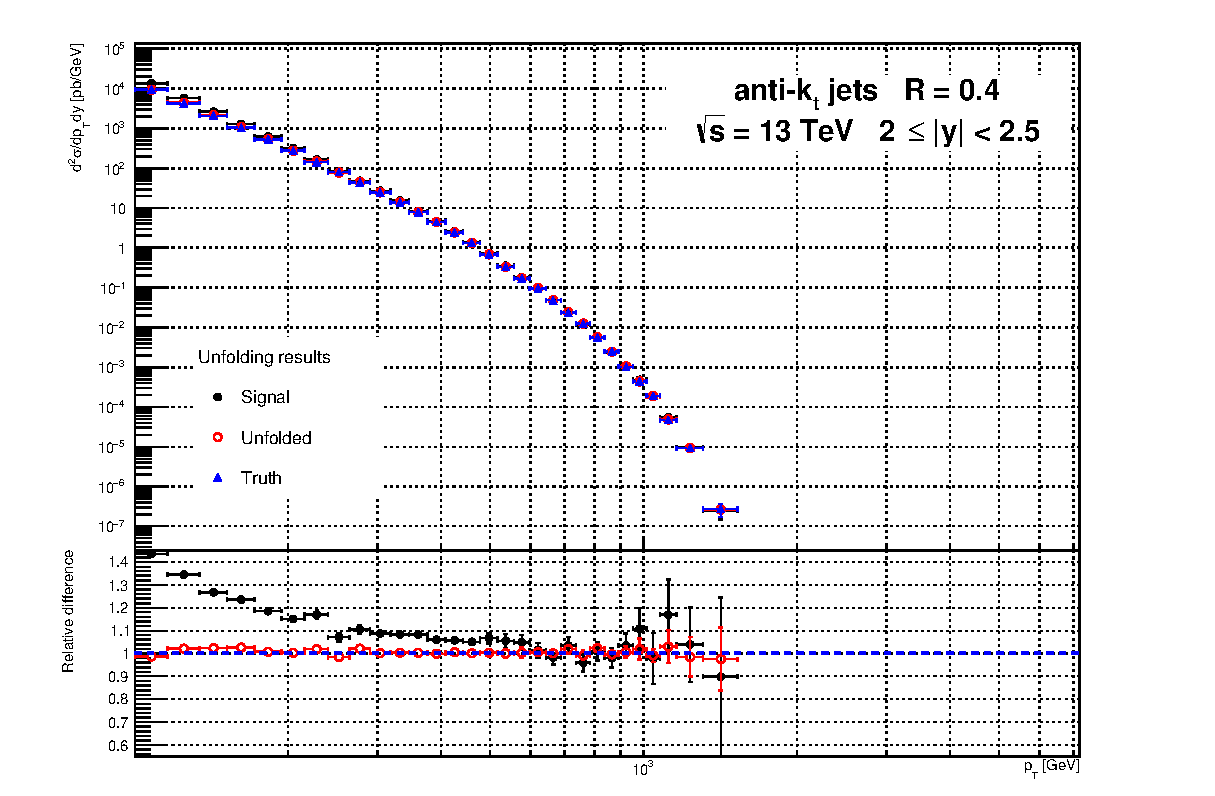
\includegraphics[width=0.9\textwidth]{{Chapter3/Signal_VS_Unfold_VS_Truth_abs(y)2-2.5}.eps}
  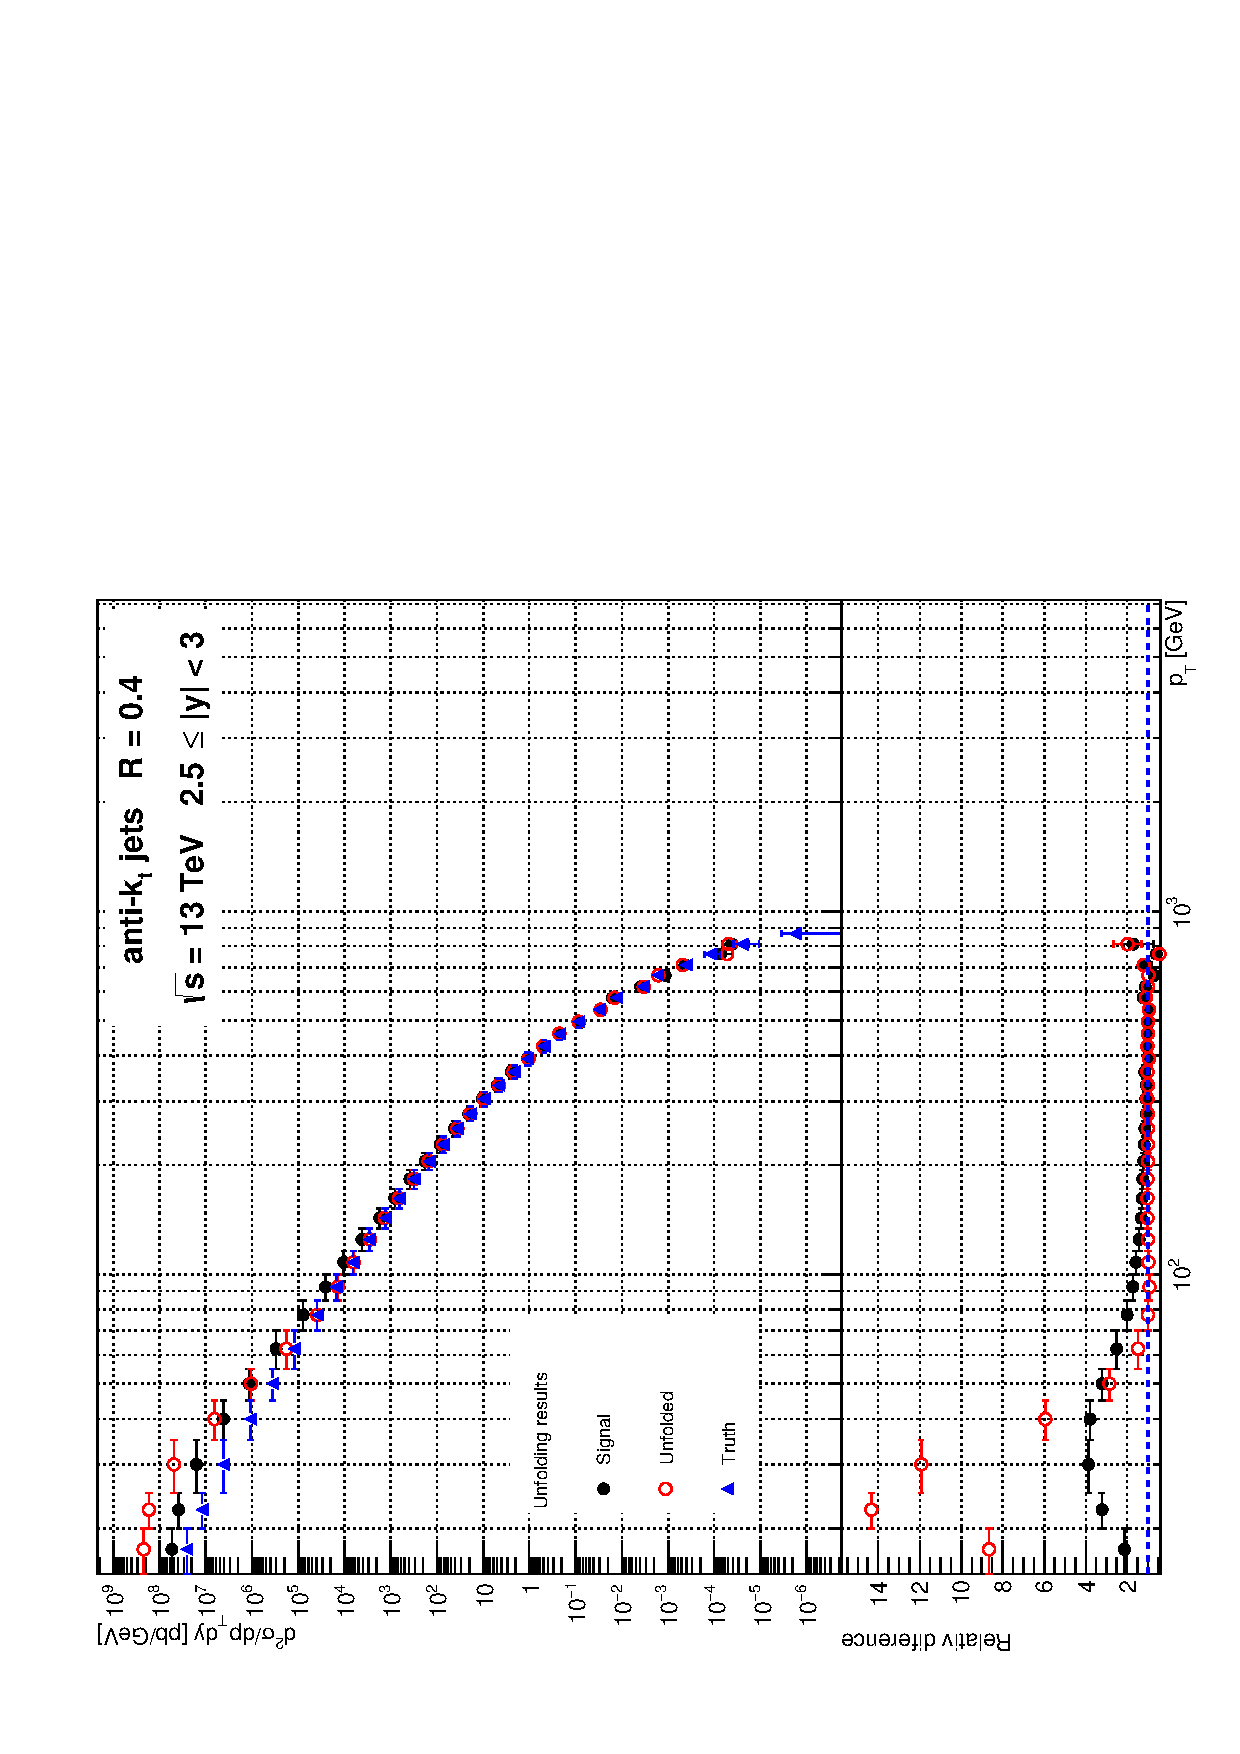
\includegraphics[width=0.9\textwidth]{{Chapter3/Signal_VS_Unfold_VS_Truth_abs(y)2.5-3}.eps}
  \caption{Comparison of spectra of signal jets and unfolded spectra of signal
  jets with the spectrum of truth jets for $2 \leq |y| < 2.5$ (top) and $2.5
  \leq |y| < 3$ (bottom) rapidity bin. Each bin was divided by its width so the
  $y$-axis has meaning of double differential cross section in $\pt$ and $y$. The
  graph at bottom shows the relative difference between signal or unfolded
  spectrum and the truth spectrum.} 
  \label{fig:Unfolding3}
\end{figure}

\begin{figure}[p]
  \centering
  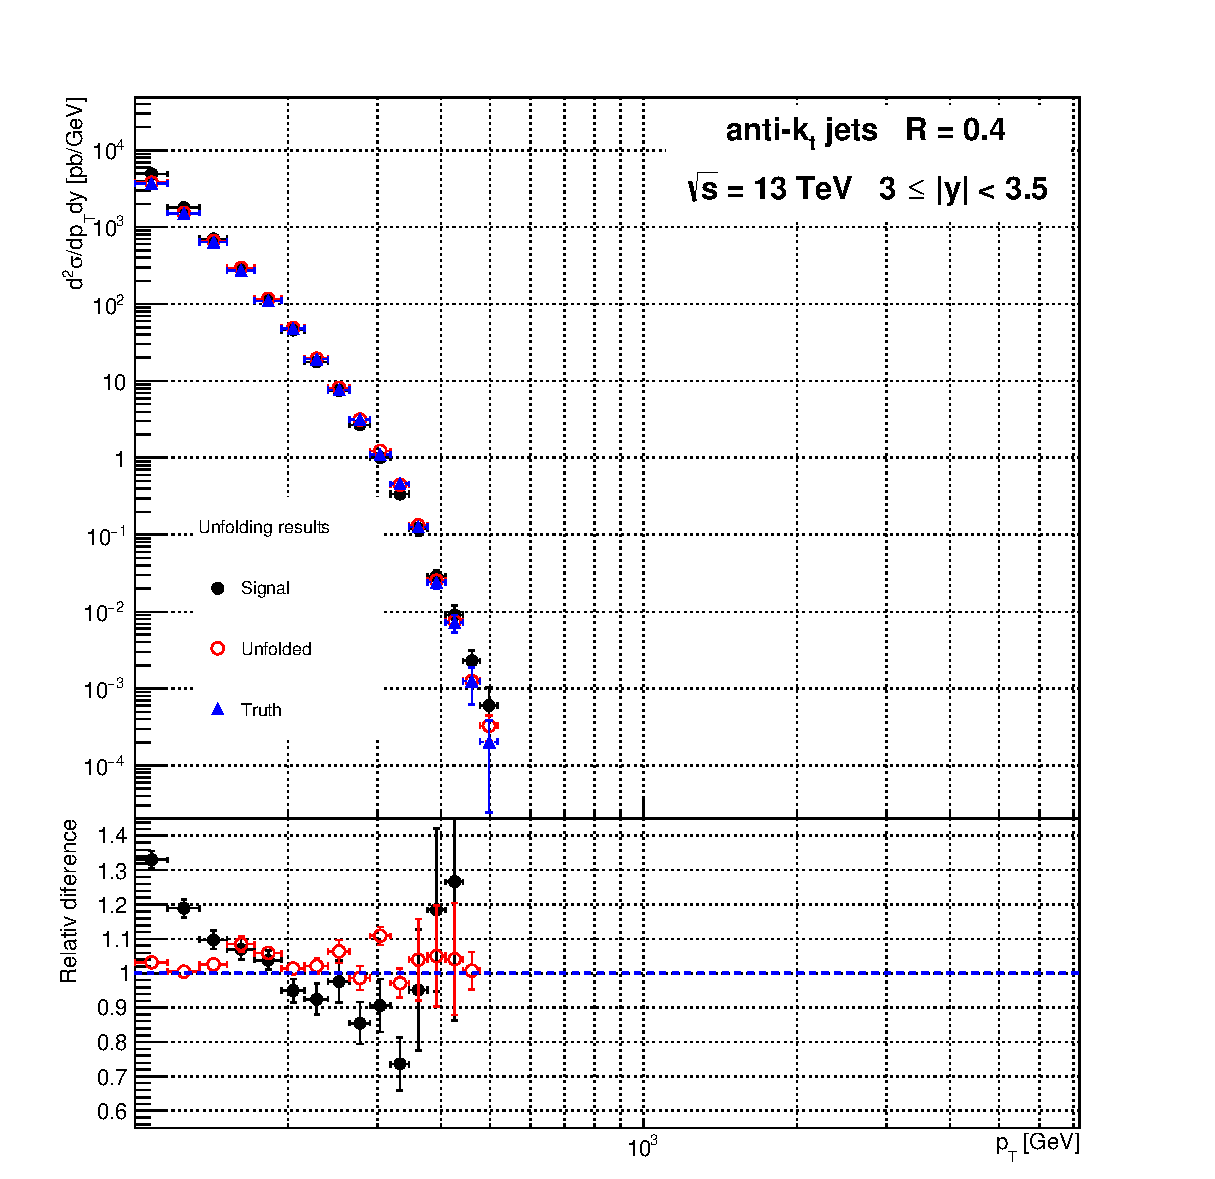
\includegraphics[width=0.9\textwidth]{{Chapter3/Signal_VS_Unfold_VS_Truth_abs(y)3-3.5}.eps}
  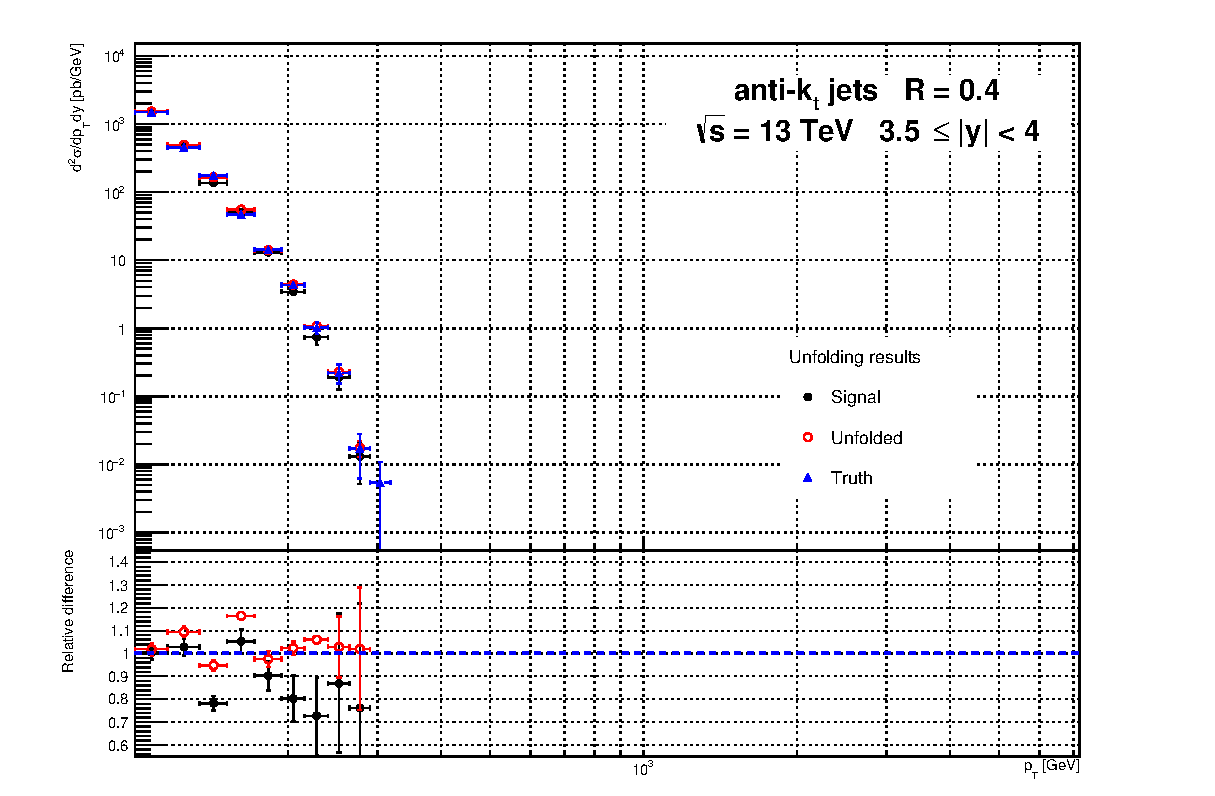
\includegraphics[width=0.9\textwidth]{{Chapter3/Signal_VS_Unfold_VS_Truth_abs(y)3.5-4}.eps}
  \caption{Comparison of spectra of signal jets and unfolded spectra of signal
  jets with the spectrum of truth jets for $3 \leq |y| < 3.5$ (top) and $3.5
  \leq |y| < 4$ (bottom) rapidity bin. Each bin was divided by its width so the
  $y$-axis has meaning of double differential cross section in $\pt$ and $y$. The
  graph at bottom shows the relative difference between signal or unfolded
  spectrum and the truth spectrum.} 
  \label{fig:Unfolding4}
\end{figure}

\chapter{Unfolding and Prediction}
\label{App:UnfoldingAndPrediction}

\begin{figure}[h]
  \centering
  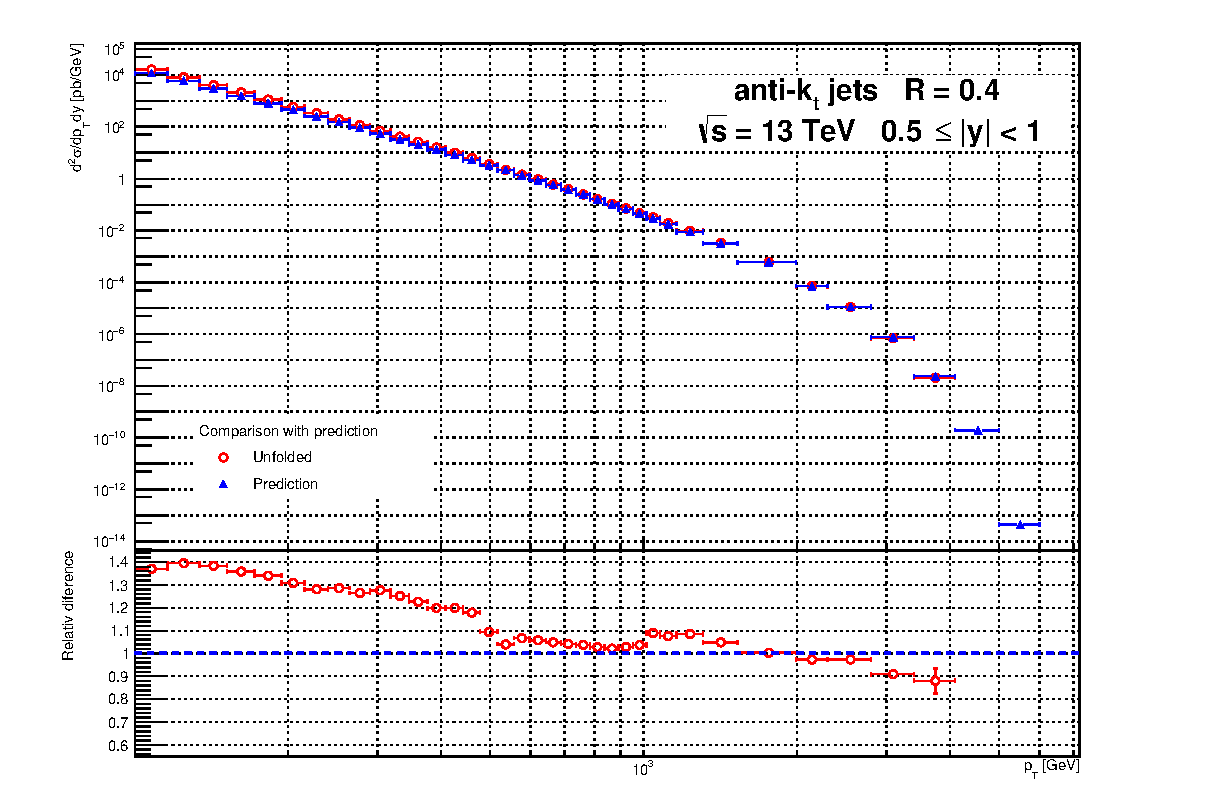
\includegraphics[width=\textwidth]{{Chapter3/Unfolded_VS_Prediciton_abs(y)0.5-1}.eps}
  \caption{Unfolded double differential cross section of inclusive jets in
  $\pt$ and rapidity $y$ compared to the NLO QCD prediction for $0.5 \leq |y| < 1$
  rapidity bin. At the bottom the relative difference between unfolded and
  predicted cross section is shown. }
  \label{fig:CompareUnfoldPred1}
\end{figure}

\begin{figure}[p]
  \centering
  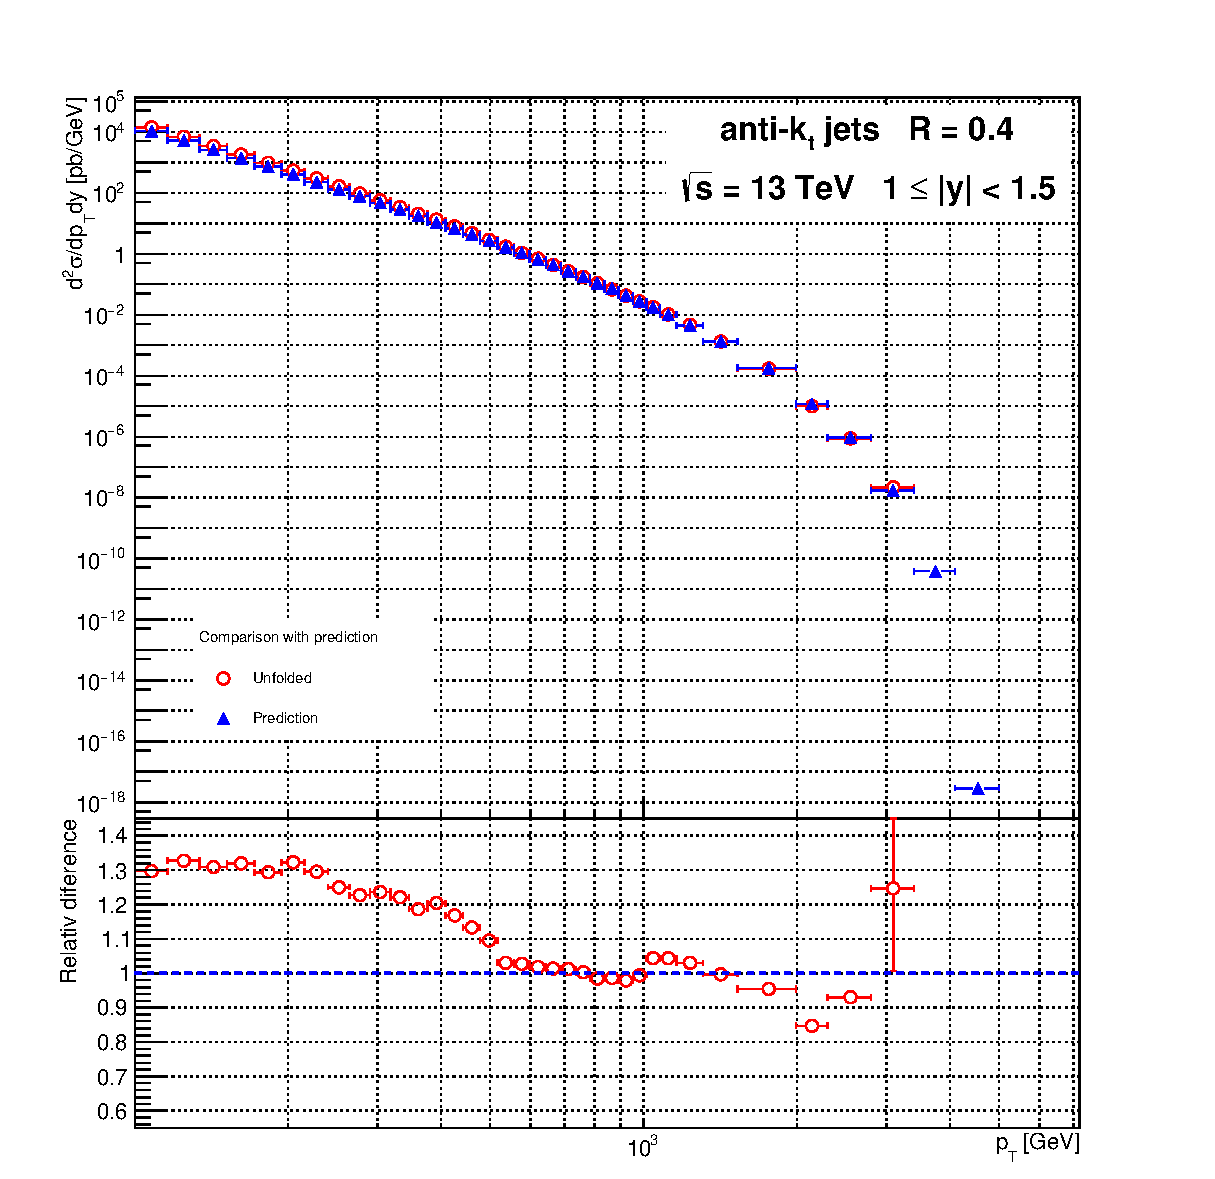
\includegraphics[width=0.9\textwidth]{{Chapter3/Unfolded_VS_Prediciton_abs(y)1-1.5}.eps}
  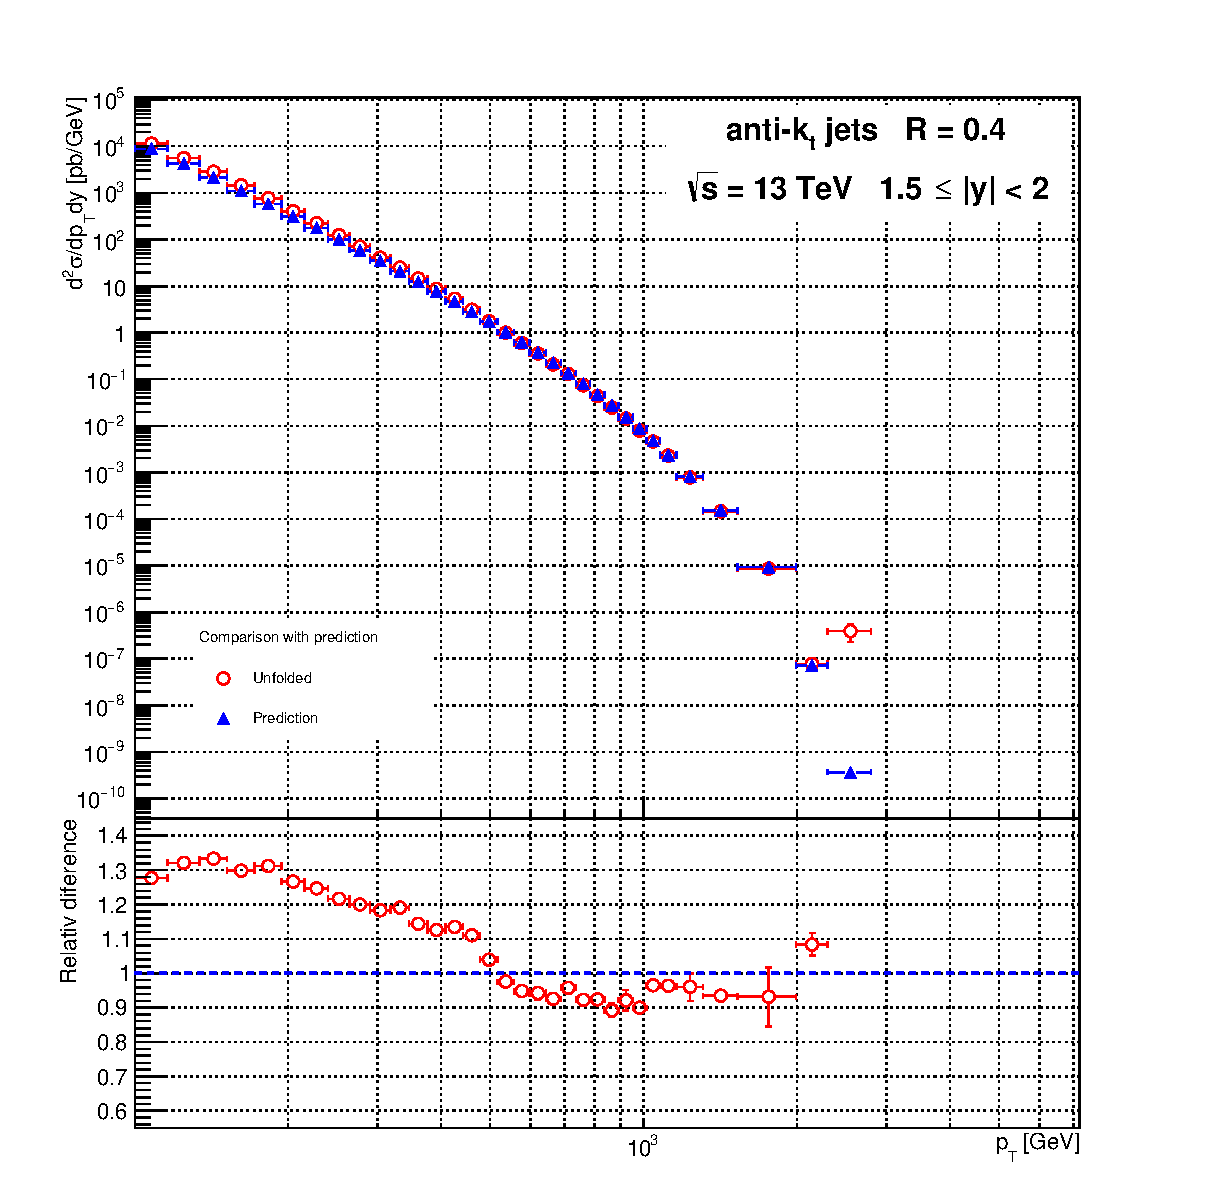
\includegraphics[width=0.9\textwidth]{{Chapter3/Unfolded_VS_Prediciton_abs(y)1.5-2}.eps}
  \caption{Unfolded double differential cross section of inclusive jets in
  $\pt$ and rapidity $y$ compared to the NLO QCD prediction for $1 \leq |y| <
  1.5$ (top) and $1.5 \leq |y| < 2$ (bottom) rapidity bin. At the bottom the
  relative difference between unfolded and predicted cross section is shown. }
  \label{fig:CompareUnfoldPred2}
\end{figure}

\begin{figure}[p]
  \centering
  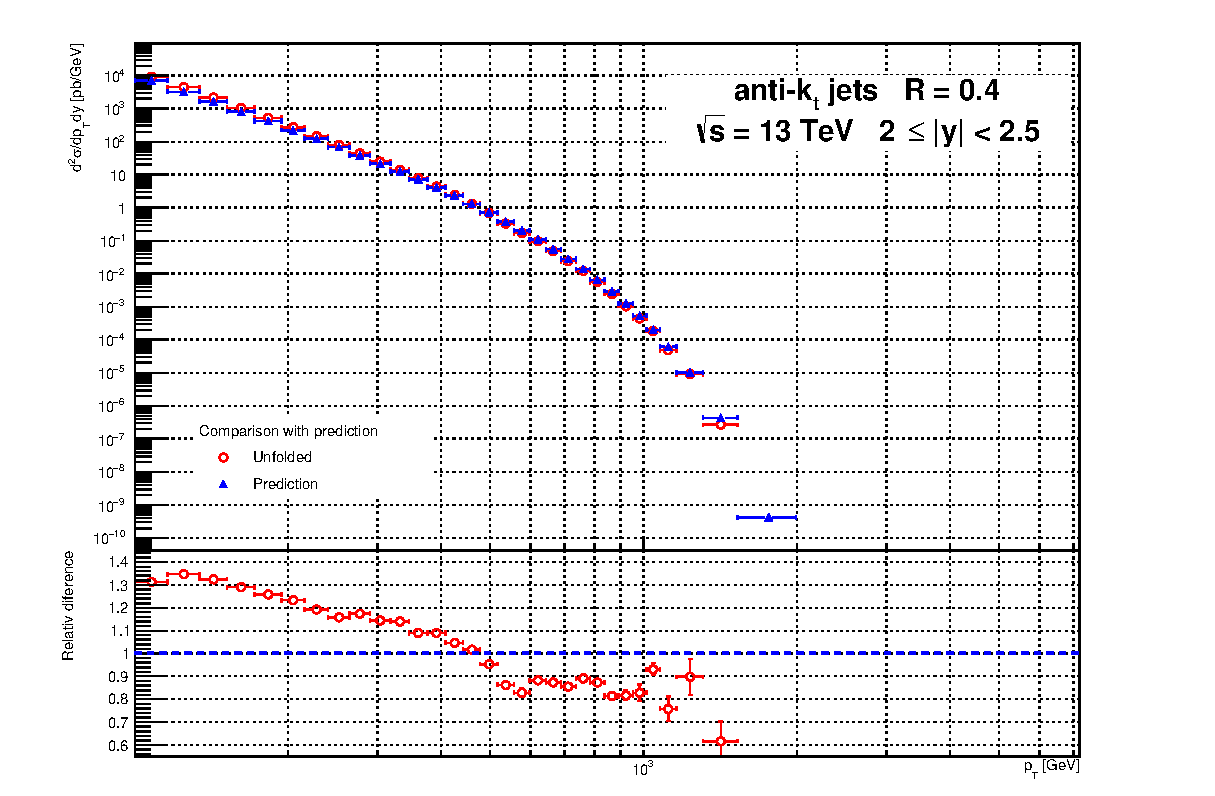
\includegraphics[width=0.9\textwidth]{{Chapter3/Unfolded_VS_Prediciton_abs(y)2-2.5}.eps}
  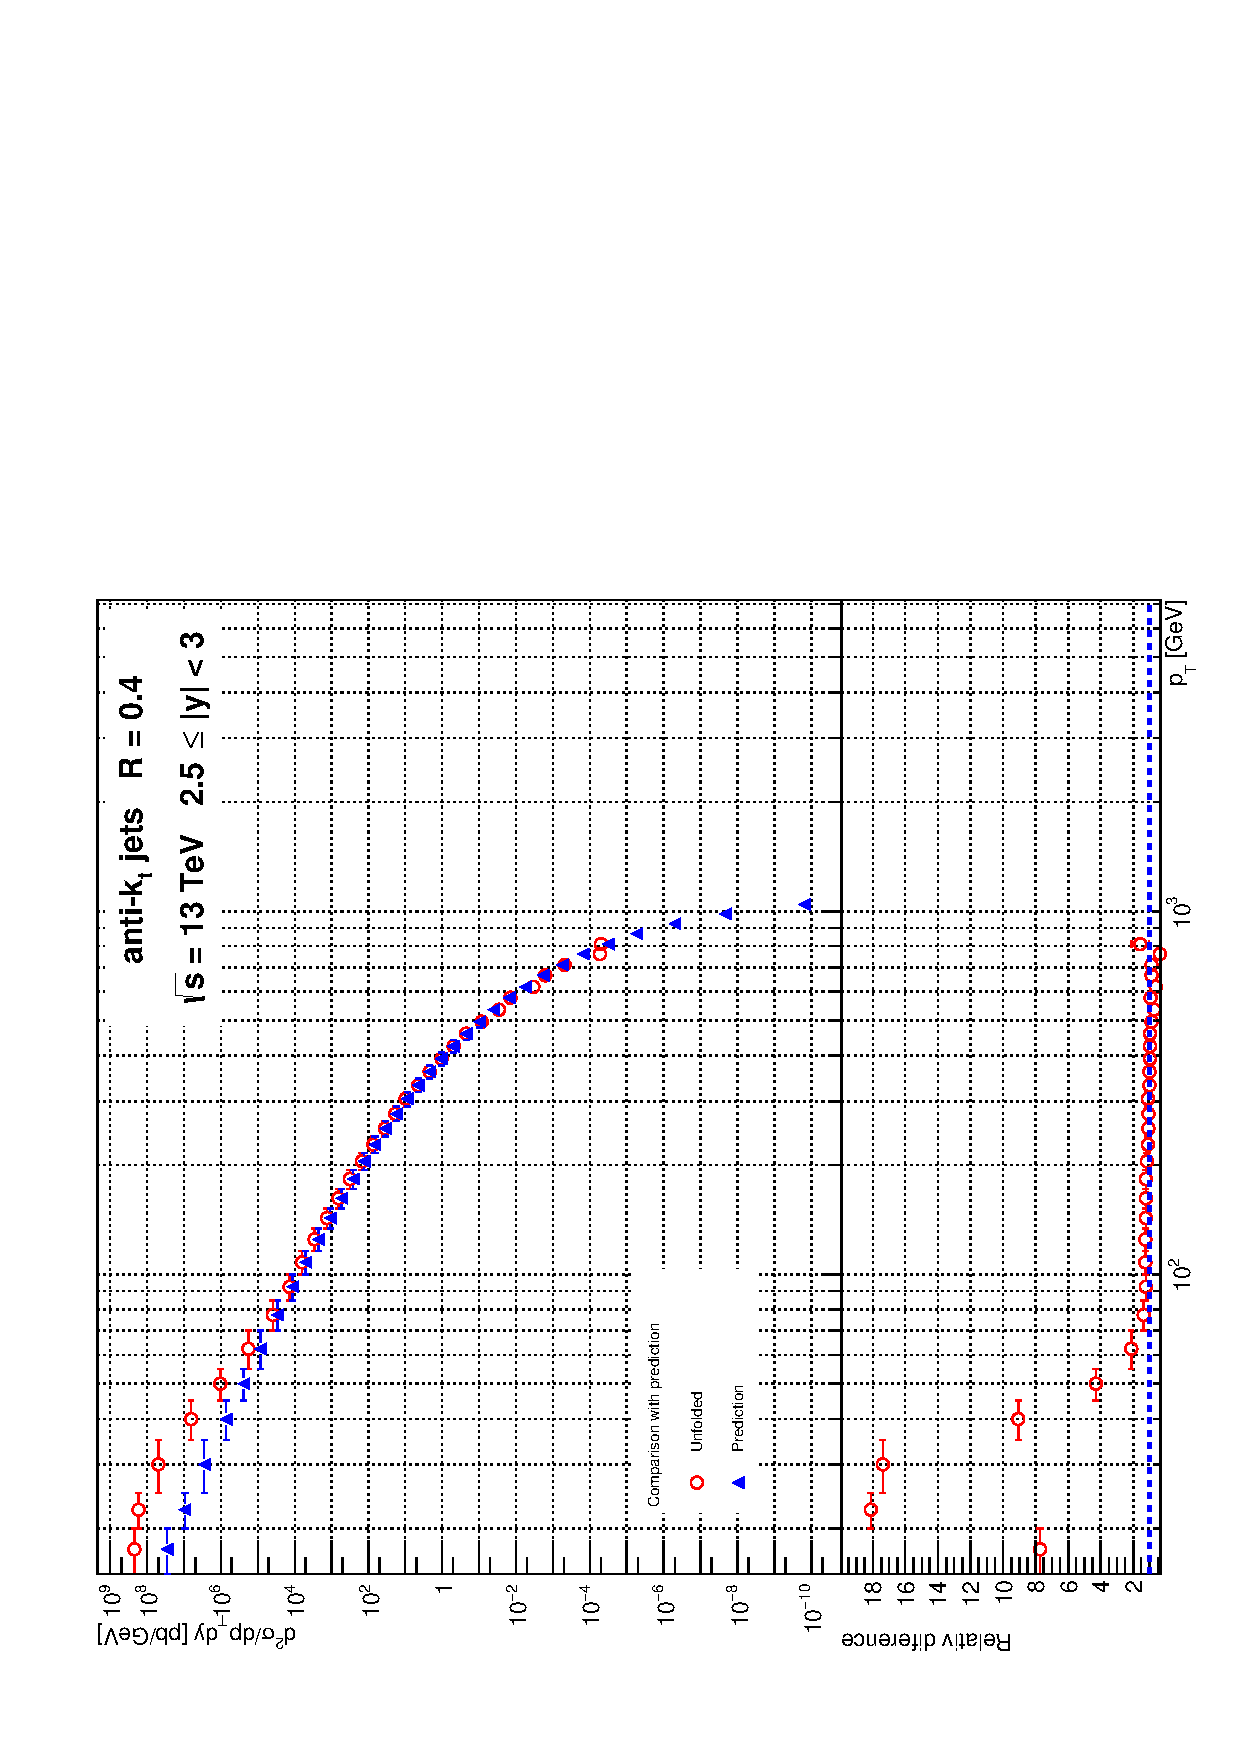
\includegraphics[width=0.9\textwidth]{{Chapter3/Unfolded_VS_Prediciton_abs(y)2.5-3}.eps}
  \caption{Unfolded double differential cross section of inclusive jets in
  $\pt$ and rapidity $y$ compared to the NLO QCD prediction for $2 \leq |y| <
  2.5$ (top) and $2.5 \leq |y| < 3$ (bottom) rapidity bin. At the bottom the
  relative difference between unfolded and predicted cross section is shown. }
  \label{fig:CompareUnfoldPred3}
\end{figure}

\end{appendices}
